\documentclass[11pt]{article}
\usepackage[utf8]{inputenc}
\usepackage[T1]{fontenc}
\usepackage{amsmath}
\usepackage{amssymb}
\usepackage{multicol}
\usepackage{geometry}
\usepackage{tikz}
\usepackage{enumitem}
\usepackage{xcolor}
\usepackage{titlesec}

% Configurações de layout
\geometry{a4paper, left=1cm, right=1cm, top=0.5cm, bottom=1.2cm}
\setlength{\columnseprule}{0.4pt}

% Cores para títulos
\titleformat{\section}{\normalfont\Large\bfseries\color{blue}}{\thesection}{1em}{}
\titleformat{\subsection}{\normalfont\large\bfseries\color{red}}{\thesubsection}{1em}{}

\title{\textcolor{red}{Primeiro Trimestre: Matemática
    \\Medidas de Tendência Central}}
\author{Professor: Jefferson}
\date{}

\begin{document}

\maketitle
\vspace{-1cm}

%\begin{center}
%\large{Nome: \underline{\hspace{8cm}} \quad Turma: \underline{\hspace{3cm}}}
%\end{center}

\begin{multicols}{2}

\section*{Fórmulas Importantes}

\subsection*{Média Aritmética}

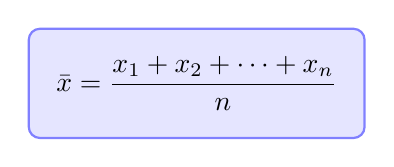
\begin{tikzpicture}
\node[rectangle, fill=blue!10, rounded corners, inner sep=10pt, draw=blue!50, thick] (box) {
$\displaystyle \bar{x} = \frac{x_1 + x_2 + \cdots + x_n}{n}$
};
\end{tikzpicture}

\textbf{Onde:}
\begin{itemize}
\item $\bar{x}$ = média aritmética
\item $x_1, x_2, \ldots, x_n$ = valores dos dados
\item $n$ = número total de dados
\end{itemize}

\subsection*{Mediana}

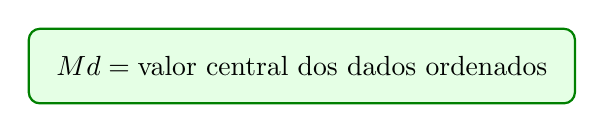
\begin{tikzpicture}
\node[rectangle, fill=green!10, rounded corners, inner sep=10pt, draw=green!50!black, thick] (box) {
$\displaystyle Md = \text{valor central dos dados ordenados}$
};
\end{tikzpicture}

\textbf{Procedimento:}
\begin{enumerate}
\item Ordene os dados em ordem crescente
\item Se $n$ é ímpar: $Md = \text{valor do meio}$
\item Se $n$ é par: $Md = \frac{\text{dois valores centrais}}{2}$
\end{enumerate}

\subsection*{Moda}

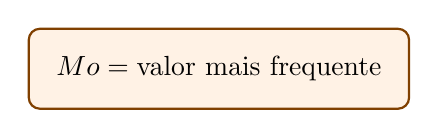
\begin{tikzpicture}
\node[rectangle, fill=orange!10, rounded corners, inner sep=10pt, draw=orange!50!black, thick] (box) {
$\displaystyle Mo = \text{valor mais frequente}$
};
\end{tikzpicture}

\textbf{Tipos:}
\begin{itemize}
\item Amodal: nenhuma moda
\item Unimodal: uma moda
\item Bimodal: duas modas
\item Multimodal: três ou mais modas
\end{itemize}

\section*{Exercícios Básicos}

\begin{enumerate}[leftmargin=*]

\item Calcule a média aritmética dos seguintes conjuntos:
\begin{enumerate}[label=\alph*)]
\item $4, 7, 9, 12, 18$
\item $8, 8, 10, 12, 14, 18$
\item $5, 10, 15, 20, 25$
\end{enumerate}

\item Determine a mediana dos conjuntos:
\begin{enumerate}[label=\alph*)]
\item $6, 2, 8, 4, 10$ (ordene primeiro)
\item $15, 20, 25, 30, 35, 40$
\item $3, 7, 1, 9, 5, 8, 2$
\end{enumerate}

\item Encontre a moda dos conjuntos:
\begin{enumerate}[label=\alph*)]
\item $4, 6, 4, 8, 4, 10, 6$
\item $12, 15, 18, 15, 20, 12, 25$
\item $7, 9, 11, 13, 15$ (classifique)
\end{enumerate}

\item Dado o conjunto: $5, 8, 8, 12, 15, 8, 20$, calcule:
\begin{enumerate}[label=\alph*)]
\item Média
\item Mediana
\item Moda
\end{enumerate}

\item Resolva os problemas:
\begin{enumerate}[label=\alph*)]
\item As alturas de 4 amigos são: 165, 170, 175, 180 cm. Qual a média de altura?
\item Se Maria tira notas 5, 6, 7, qual deve ser sua 4ª nota para ter média 6,5?
\end{enumerate}

\item Analise e compare os conjuntos:

\textbf{Conjunto A:} $12, 14, 16, 18, 20$

\textbf{Conjunto B:} $12, 12, 12, 20, 24$

\begin{enumerate}[label=\alph*)]
\item Calcule média, mediana e moda de cada
\item Qual conjunto é mais homogêneo?
\end{enumerate}

\item Problemas contextualizados:
\begin{enumerate}[label=\alph*)]
\item Um jogador fez nos últimos 5 jogos: 8, 12, 6, 10, 14 pontos. Qual sua média?
\item As idades de uma família: 12, 15, 18, 42, 45 anos. Encontre as 3 medidas.
\end{enumerate}

\item Identifique em cada caso qual medida é mais adequada:
\begin{enumerate}[label=\alph*)]
\item Salários de uma empresa pequena
\item Notas de uma prova difícil
\item Cor de camiseta mais popular na escola
\end{enumerate}

\item Calcule as três medidas para:
\begin{enumerate}[label=\alph*)]
\item $10, 15, 20, 25, 30, 35, 40$
\item $3, 4, 4, 5, 6, 6, 6, 7, 8$
\item $50, 60, 70, 80, 90$
\end{enumerate}


\section*{Dicas para Resolver}

\begin{itemize}
\item \textbf{Média}: Some todos os valores e divida pela quantidade
\item \textbf{Mediana}: SEMPRE ordene os dados primeiro
\item \textbf{Moda}: Valor que mais se repete (pode ter mais de uma)
\item \textbf{Dados agrupados}: Use ponto médio × frequência para média
\item \textbf{Comparação}: Média é sensível a valores extremos
\end{itemize}


\end{multicols}

\end{document}
